% Space SHAP manuscript, target: npj Microgravity (collection: Human System Risk
% Management and Knowledge Graphs for Human Spaceflight, Vol. II).
%
% Provenance and rules (ADR 009):
%   - The Introduction is HUMAN-WRITTEN, reproduced verbatim from the August
%     2026 Word draft. Revise it by hand only. An LLM may suggest; it never
%     rewrites. Nature journals restrict LLM-written text.
%   - Blocks marked \draftnote{...} were drafted with an LLM from the
%     project's own records and must be rewritten by a human before
%     submission. Blocks marked \todo{...} are open items.
%   - Methods follow the 13-step flow of the original repository.
%   - Nothing gated by Lucidity Sciences' sign-off (ADR 008) appears here.
%
% Build: latexmk -pdf main.tex   (or `make manuscript` from the repo root)

\documentclass[11pt]{article}
\usepackage[margin=1in]{geometry}
\usepackage[T1]{fontenc}
\usepackage[utf8]{inputenc}
\usepackage{lmodern}
\usepackage{amsmath,amssymb}
\usepackage{graphicx}
\usepackage{booktabs}
\usepackage{xcolor}
\usepackage[numbers,sort&compress]{natbib}
\usepackage[hidelinks]{hyperref}
\usepackage{caption}
\captionsetup{font=small,labelfont=bf}
\graphicspath{{../docs/images/}}

\newcommand{\todo}[1]{\textcolor{red!70!black}{[TODO: #1]}}
\newcommand{\draftnote}[1]{\textcolor{blue!60!black}{[LLM draft, rewrite by hand: #1]}}
\newcommand{\dox}{\operatorname{do}}

\title{A playbook for graph-based intervention estimation:\\
prediction is the default, intervention casts a wider net\\
\large A known-truth study on NASA's renal-stone topology}
\author{Andy Wilson \and Lexi Pasi \and Robert J. Reynolds \and Aimee Harrison\\[4pt]
\normalsize\todo{author list and order unconfirmed; affiliations}}
\date{Working draft, \today}

\begin{document}
\maketitle

\begin{abstract}
\draftnote{abstract}
Machine-learning explanations such as SHAP are increasingly read as maps of
where to intervene. On a causal graph that reading fails in a specific way:
a mediator can screen off its ancestors for prediction while still
transmitting their intervention effects, so predictive credit pools near the
outcome and the upstream nodes an intervention would have to touch drop out
of the ranking. We treat prediction and intervention as different goals with
different recipes, and we test a playbook for the second on synthetic data
generated from NASA's Human System Risk Board renal-stone DAG (SA-07566),
where the total effect of every node is known by construction. Two scales of
the same graph are used: a 14-node working subgraph and the full 51-node
source graph. Standard SHAP, run across five explainer and model pairings,
inverts a two-hop mediation chain in four of the five. Supplying a causal
ordering to the attribution method does not repair the ranking (Kendall's
$\tau$ 0.528 against 0.506 for matched ordinary SHAP, paired-bootstrap
interval covering zero), while propagating interventions through the
structural model does ($\tau$ 0.794, top-five recovery 1.00, a prototype).
A discovery-based method returned all zeros until an expert reconnected the
outcome that PC had pruned at $n=1{,}000$, and reached $\tau$ 0.714 once it
was. We show analytically and by simulation that deeper nodes wash out first
as sampling variance grows, state the working assumption that direct
relationships are close to linear, and lay out the two placeholder rungs the
playbook needs to fill: a detector for depth and a two-channel filter for
noise. All data are synthetic; NASA supplies topology, not effects.
\end{abstract}

% =====================================================================
\section{Introduction}
% ---------------------------------------------------------------------
% HUMAN-WRITTEN. Verbatim from "Space SHAP_ Intro & Methods Drafts.docx"
% (2026-08-10) as snapshotted 2026-08-11. Citation keys were substituted for
% the parenthetical author-year strings; entries marked TODO in
% references.bib still need checking against the sources.
% ---------------------------------------------------------------------

\todo{Andy's note from the draft: ``I had Claude add citations where I was
going off the book. I need to check all citations.'' Keys marked TODO in
\texttt{references.bib}.}

Understanding the complex, interrelated pathways between spaceflight
environmental hazards and multiple mission-level outcomes is a critical need
to support future deep space travel \citep{Reynolds2022,NASA2022DAGs}.
Spaceflight data sets present unique challenges for epidemiological research
and risk assessment modeling due in part to their sparseness and inherent
selection bias \citep{ReynoldsDay2019a,Reynolds2023}; recent innovations in
predictive and statistical methods provide promising remedies to these
limitations \citep{Li2023,Sanders2023,Scott2023}. However, application of
novel methods without well-informed, causal reasoning may lead to naive
calculations that are confidently backed by data but not by realistic
mechanisms \citep{HookerMentch2019,Reisach2021}; this is particularly true
when the methods employ machine learning (ML).

In support of causally motivated research, the Human System Risk Board
(HSRB) team at the National Aeronautics and Space Administration (NASA)
maintains expert-driven directed acyclic graphs (DAGs) for the approximately
30 known spaceflight risks \citep{Antonsen2024}. In addition to providing
justifiable, foundational models that are easily communicated between
researchers, DAGs also codify causal relationships in a manner that is
interpretable to machines; they are used as baseline data for many causal
packages and predictive models \citep{Kalisch2012,Textor2016,SharmaKiciman2020}.
The lifecycle of these DAGs includes human review as well as data-driven
validation; explicitly defined metrics and evaluation procedures weight
evidence from multiple sources to evaluate effect strength and to affirm and
refine the edges in NASA's maintained DAGs \citep{Reynolds2022,Antonsen2023,Ward2024}.

Explainable AI (XAI) has emerged to make the behavior of otherwise opaque ML
models transparent, offering methods applied after a model is trained, which
quantify how individual input features contribute to its predictions
\citep{BarredoArrieta2020,ViloneLongo2021}. Based on Shapley values, a
cooperative game-theory method for fairly distributing a payout among the
players who produce it, SHAP treats each input feature as a player and
assigns it the marginal contribution it makes to a given prediction, yielding
additive and locally accurate feature attributions
\citep{LundbergLee2017,Shapley1953}. Out of the box SHAP and similar
algorithms derive feature importance without a causal framework;
epidemiology teams increasingly interpret these outputs to inform causal
pathways and to guide study design and statistical analyses
\citep{Lundberg2020,AnnalsEpi2025}. XAI algorithms, such as SHAP, offer a
data-driven approach to validate and enhance these diagrams.

However, out of the box SHAP does not see causal structures and thus can
identify spurious relationships and underweights downstream effects in favor
of features proximate to the outcome
\citep{ACIC2026,Janzing2020,Aas2021,Kumar2020,Ng2025}. Because these
attributions carry the errors noted above, their interpretation risks
incorrect causal conclusions unless paired with critical human oversight.
Causally informed SHAP, by contrast, is aware of the causal structure, which
provides opportunities for capturing feature importance and effect strength
with higher fidelity \citep{Ng2025}.

\todo{From the draft: write the paragraph on what causally informed SHAP is
and overview each individual method and its dependency on the DAG. The
Methods section below (Step 6) has the material.}

To our knowledge, no prior work has applied causal feature-attribution
methods to human spaceflight epidemiology, nor systematically benchmarked
out-of-the-box SHAP against causally informed variants under the data
constraints characteristic of astronaut cohorts. This gap is one the
architects of NASA's DAG program have themselves flagged; machine learning
has been named as a priority future direction for populating and refining
the risk DAGs \citep{Reynolds2022,Sanders2023}. By evaluating how well a
validated ground-truth DAG can be recovered under both full and partial
specification, as well as under progressive degradation toward realistic
spaceflight data conditions, this work directly addresses that need and
offers a reusable template for causally faithful attribution in sparse,
highly selected cohorts.

\todo{From the draft, to finalize once scope is settled: ``This paper offers
a systematic evaluation of the results of out of the box SHAP versus
causally informed SHAP variants, evaluated against a ground truth. Using
synthetic data, seeded with DAGs from NASA's maintained library, we will
consider how well multiple frameworks and multiple engines can recover a DAG
with either full or partial initial specification.''}

% ---------------------------------------------------------------------
\subsection*{Two goals, two playbooks}
\draftnote{this subsection is new framing from the 1 September 2026 notes
and the framing memo (docs/framing); it needs a human rewrite before it
joins the human-written paragraphs above}

Modeling for prediction and modeling for intervention are different jobs
with different recipes. The split is standard in statistics and
epidemiology \citep{Shmueli2010,Hernan2019,Harrell2015}. Explainable AI runs
the prediction recipe by default: fit the best predictor, explain it, read
the ranking as a list of what matters. That default is adequate for
prediction. For intervention it fails structurally, because a mediator can
screen off its ancestors for prediction while still transmitting their
effects. The intervention playbook therefore has to cast a wider net,
deliberately re-admitting candidate nodes the predictor discarded, and then
prune that wider set with structural reasoning rather than with predictive
importance.

The wider net is where the difficulty lives. Deeper nodes carry smaller
total effects, because in a linear structural model the total effect is a
sum over directed paths of the product of edge coefficients
\citep{Wright1934,Bollen1987,Sobel1987}; the sample size needed to detect a
product of coefficients rises steeply as either factor shrinks
\citep{FritzMacKinnon2007}; measurement error in a mediator biases the
indirect effect through it toward the null \citep{VanderWeele2012,Hutcheon2010};
and constraint-based discovery needs a floor on the strength of every
dependence it is asked to find \citep{ZhangSpirtes2003,Uhler2013}. The
question the playbook has to answer is therefore not ``which node is
important'' but ``how do we know a deep node from a shallow one when the
data alone make them look alike?'' This article lays out the playbook, tests
its established rungs on two scales of NASA's renal-stone topology with a
known answer key, and specifies the two rungs that remain to be filled.

% =====================================================================
\section{Results}

\subsection{The known world}
\draftnote{Results are assembled from docs/step04\_results.md,
docs/step06\_results.md, and docs/full\_dag/RESEARCH\_RECORD.md; every
number is traceable to a frozen artifact in the repository}

The primary case study is a 14-node working subgraph scoped from NASA's
SA-07566 renal-stone DAG (Fig.~\ref{fig:dag}), with cumulative mission
duration as the exposure and nephrolithiasis (binary incidence) as the sole
outcome. Every edge carries its evidence status from the NASA narrative and
the literature; every coefficient is a simulation design parameter, not a
NASA effect estimate. Data were generated with \texttt{simcausal}
\citep{Sofrygin2017} at $n=1{,}000$ (seed 20260812), and the interventional
total effect of each of the 13 candidate features on $P(\text{nephrolithiasis})$
was computed before any attribution method ran, as
$\mathbb{E}[Y\mid\dox(X=\text{hi})]-\mathbb{E}[Y\mid\dox(X=\text{lo})]$ over
50{,}000 common-random-number draws. The full 51-node source graph (75 edges,
Cohen's $\kappa=1.000$ against the published DAGitty code) was simulated
the same way at $n=10{,}000$, with frozen truth for its 28 ancestors of the
outcome.

\begin{figure}[htbp]
\centering
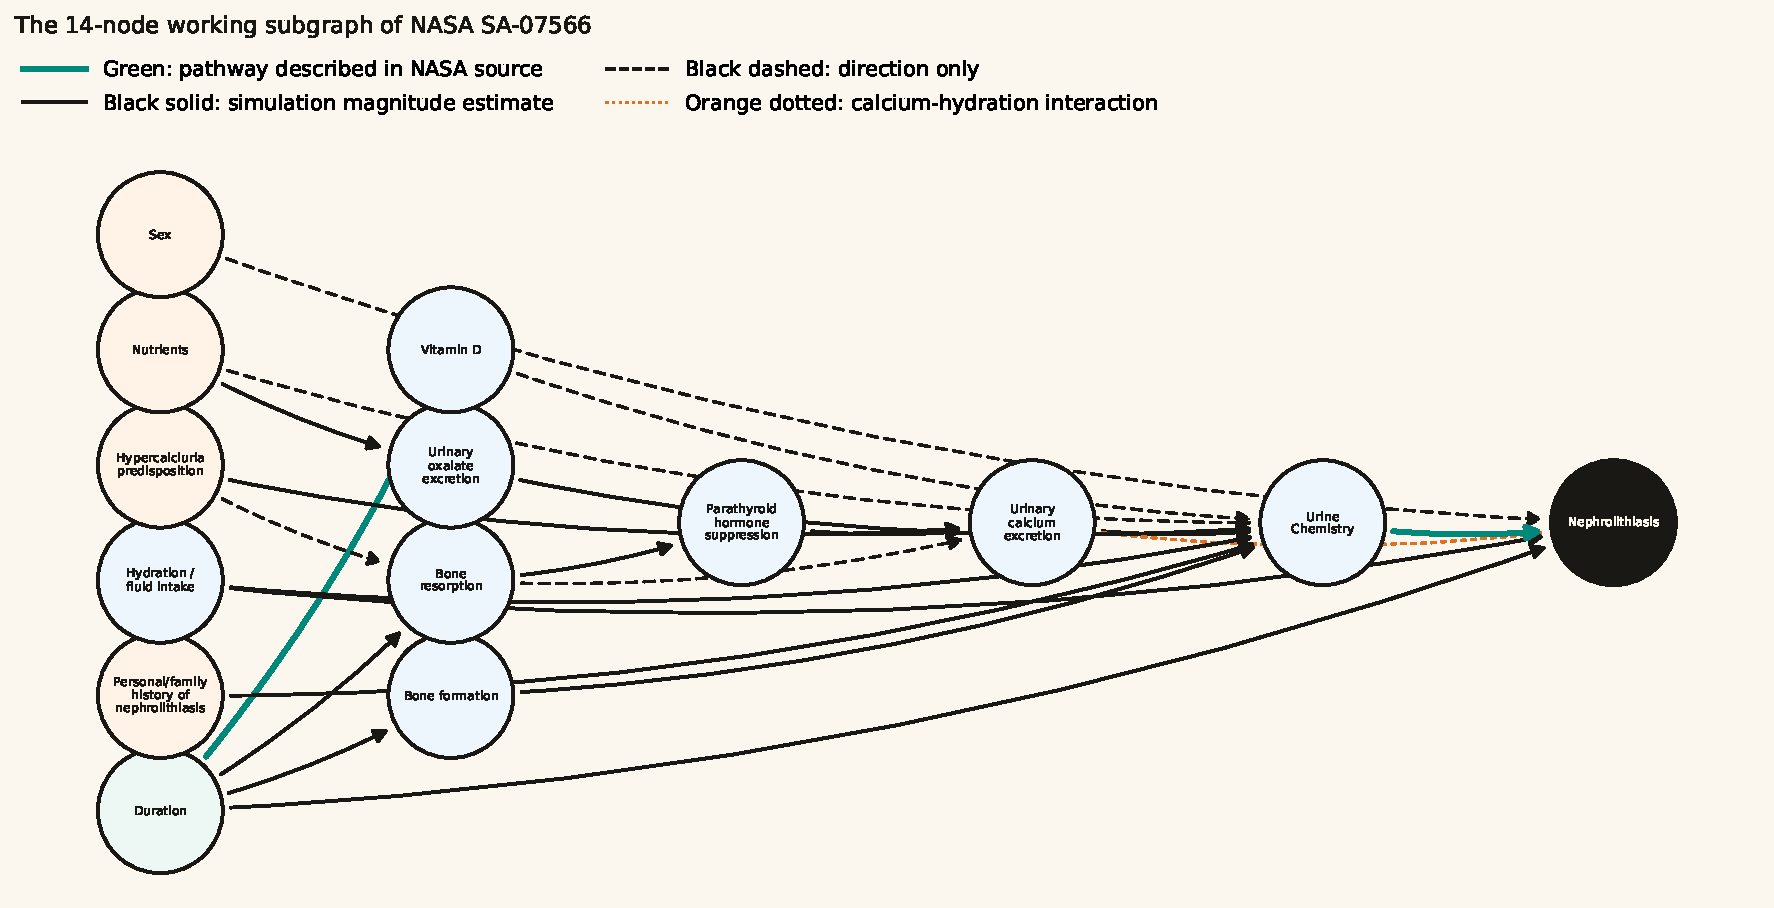
\includegraphics[width=\textwidth]{working_subgraph_dag.pdf}
\caption{The 14-node working subgraph of NASA SA-07566. Edge style follows
the evidence status recorded in \texttt{config/dag\_spec.yaml}; the orange
dotted edge is the urinary-calcium by hydration interaction. Mineralized
renal material (calcium-oxalate supersaturation) is collapsed onto the
outcome because it was the outcome's only parent, which would have let any
method trivially place all credit on one node.}
\label{fig:dag}
\end{figure}

\subsection{The prediction playbook, done well, inverts a mediation chain}

Five explainer and model pairings were run on the same data
(Table~\ref{tab:step4}). Every pairing's rank agreement with the frozen
truth fell when the graph gained real mediation depth (from an earlier
11-node version to the 14-node one), and the ordering of methods reshuffled:
the linear explainer led on the shallow graph and fell to second-to-last on
the deeper one, where correlated mediators divide credit more sharply in a
logistic regression than in a tree ensemble.

\begin{table}[htbp]
\centering
\caption{Step 4. Kendall's $\tau$ between each pairing's global importance
(mean $|$SHAP$|$ on the held-out test set) and the frozen interventional
truth, on the earlier 10-feature and the current 13-feature working
subgraph.}
\label{tab:step4}
\begin{tabular}{llrr}
\toprule
Explainer & Engine & $\tau$ (10 features) & $\tau$ (13 features)\\
\midrule
TreeExplainer (interventional) & random forest & 0.689 & 0.359\\
PermutationExplainer & XGBoost, black box & 0.556 & 0.308\\
TreeExplainer (interventional) & XGBoost & 0.422 & 0.282\\
LinearExplainer (empirical covariance) & logistic regression & 0.733 & 0.231\\
KernelExplainer & XGBoost, black box & 0.467 & 0.205\\
\bottomrule
\end{tabular}
\end{table}

The cleanest failure is on the chain nutrients $\rightarrow$ urinary oxalate
excretion $\rightarrow$ urine chemistry. In the generating process the
mediator is slightly more important than its own parent (ratio 1.28, one hop
closer to the outcome). Four of the five pairings invert this, crediting the
parent over its mediator by 1.3 to 2.6 times: mediated effect misattributed
back onto the distal node. Only the random-forest tree explainer recovered
the ratio, and on one seed that is a coincidence to be treated skeptically.
On the parallel chain bone resorption $\rightarrow$ parathyroid suppression
$\rightarrow$ urinary calcium excretion every pairing got the direction
right but the linear explainer overshot the ratio by more than three times
(6.39 against 1.97). A fan-out confounder (hypercalciuria predisposition,
reaching the outcome through two paths) was placed within two ranks of its
true position by every pairing: clean fan-out confounding is an easier case
for the prediction playbook than a genuine two-hop mediation chain.

\subsection{Causal SHAP with an expert in the loop}

Three causally informed methods were run over three revision rounds
(Table~\ref{tab:step6}): asymmetric Shapley values with a depth-tier causal
ordering \citep{Frye2020}, Shapley Flow \citep{Wang2021}, and the
discovery-based Causal SHAP of \citet{Ng2025} implemented from its Algorithm~1
with PC and IDA \citep{Kalisch2012}. Round one used each method's genuinely
naive input. Rounds two and three applied a scripted revision heuristic
standing in for the expert; no human reviewed them, and every round-two and
round-three number carries that label. The Heskes-style causal Shapley
values \citep{Heskes2020} could not be run through \texttt{shapr}, which
hung whenever a confounding structure was supplied; the intervention-propagating
value function described below is its replacement.

\begin{table}[htbp]
\centering
\caption{Step 6. Kendall's $\tau$ against the frozen truth on the working
subgraph, round one (naive input) and round three (after two scripted
revisions). The best causality-blind pairing from Table~\ref{tab:step4}
reached 0.359.}
\label{tab:step6}
\begin{tabular}{llrr}
\toprule
Method & Engine & $\tau$ round 1 & $\tau$ round 3\\
\midrule
Causal SHAP (Ng et al.) & XGBoost & undefined (all zero) & 0.714\\
Causal SHAP (Ng et al.) & random forest & undefined (all zero) & 0.714\\
Asymmetric Shapley values & XGBoost & 0.231 & 0.205\\
Shapley Flow & XGBoost & 0.077 & 0.154\\
\bottomrule
\end{tabular}
\end{table}

The discovery-based method's round one is a finding, not a bug. PC with a
Gaussian partial-correlation test at $\alpha=0.05$ found thirteen adjacent
feature pairs and zero edges touching the binary outcome: every marginally
significant association was pruned once the algorithm conditioned on the
urine-chemistry hub. With no path to the outcome, every weight in
Algorithm~1 is zero and the method correctly reports nothing. Once the
outcome was reconnected it reached the best rank agreement of any method
in the study. Discovery quality is the whole game for that route, and a
mixed graphical model that treats the binary node as its own type
\citep{Sedgewick2016,Sedgewick2019} is the natural next run.

\subsection{Ordering alone does not fix it; propagation does}

On the full 51-node graph, with one XGBoost model shared across methods
(held-out AUC 0.684 against a structural ceiling of 0.701), restricting the
Shapley permutations to a causal order is statistically tied with matched
ordinary SHAP (Table~\ref{tab:fulldag}). The paired bootstrap over 2{,}000
draws gives a difference in $\tau$ of 0.008 with interval $[-0.011, 0.027]$,
and the intervals for the proximity-bias index, the proximal
over-attribution area, and proximal mass all include zero. Changing the
coalition value function to $v(S)=\mathbb{E}[f(X)\mid\dox(X_S=x_S)]$, with
background observations abducted to exogenous draws and each intervention
propagated through descendants before scoring, moves the ranking toward the
truth. That result is a 32-record, 32-background, 32-permutation prototype
without repeated-seed uncertainty and is labeled as such.

\begin{table}[htbp]
\centering
\caption{Full 51-node graph. Rank agreement and proximity bias against
frozen truth for the 28 ancestors of nephrolithiasis. PBI is the
attribution-weighted mean directed distance under truth minus under the
method; positive means credit pooled too close to the outcome. The truth
places 42.1\% of importance within two hops.}
\label{tab:fulldag}
\begin{tabular}{lrrrr}
\toprule
Method & $\tau$ & Top-5 recovery & PBI & Mass within 2 hops\\
\midrule
Exact TreeSHAP & 0.522 & 0.60 & 1.082 & 83.1\%\\
Matched ordinary interventional SHAP & 0.506 & 0.60 & 1.051 & 81.6\%\\
DAG-asymmetric ordering & 0.528 & 0.60 & 1.051 & 81.2\%\\
Structural propagation (prototype) & 0.794 & 1.00 & $-0.113$ & 38.1\%\\
\bottomrule
\end{tabular}
\end{table}

On a five-node teaching graph where the total effects are exact, ordinary
SHAP put 45.6\% of its credit on a node caused by the outcome whose total
effect is zero. That example is pedagogic and is never used as evidence
about the renal topology.

\subsection{Deeper nodes wash out first}

The wider net admits deeper nodes, and three effects compound against them.
Fig.~\ref{fig:washout} isolates the first: on a standardized linear chain
with the same coefficient on every edge, the chance of detecting a node at
all falls with sample size fastest for the deepest nodes. The depth-five
node needs a sample roughly sixty times larger than the depth-one node to
reach the same power; at astronaut-cohort sizes it is gone while the
shallow layers remain. Measurement error on the mediators and the
conditioning-set growth inside constraint-based discovery make it worse,
and the disconnected outcome in Table~\ref{tab:step6} is that third effect
observed live.

\begin{figure}[htbp]
\centering
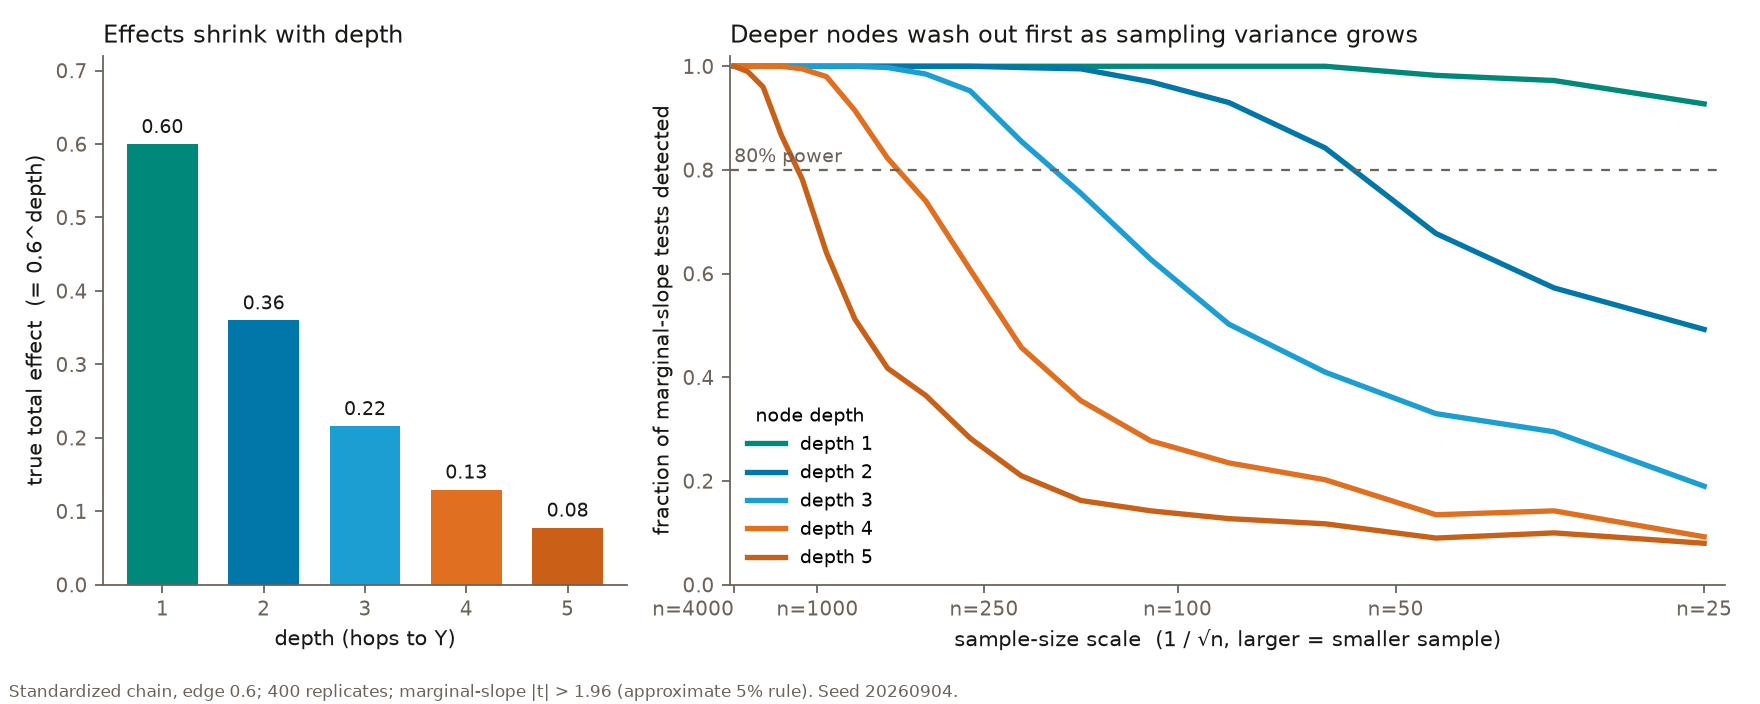
\includegraphics[width=\textwidth]{depth_washout.png}
\caption{Deeper nodes wash out first as sampling variance grows. Left: on a
standardized chain with coefficient 0.6 on every edge, the true total
effect of the node at depth $d$ is $0.6^d$. Right: the fraction of 400
replicate datasets in which the marginal slope of the outcome on the node
rejects at $\alpha=0.05$, against sampling standard error. Seed 20260904;
\texttt{analysis/depth\_washout\_figure.py}.}
\label{fig:washout}
\end{figure}

\subsection{Learned versus known: the evaluation the playbook needs}
\draftnote{Step 8 has infrastructure but no renal runs yet; this subsection
describes the battery and shows the schematics, and its results table is a
placeholder}

When the graph itself is learned from data, concordance with the sealed
graph is not the question that matters. Fig.~\ref{fig:spine} lays out the
spine: the known world is sealed before any learning, the data go through
discovery, a versioned expert ledger, and a plausible graph, and the
learned graph is judged on two axes before attribution is computed under
both graphs. Fig.~\ref{fig:m3} makes the second axis concrete. A learned
graph can have a pathway edge reversed and still yield a valid adjustment
set for the target parameter; only sufficiency transfer (M3), parameter
fidelity (M4), and identification honesty over the CPDAG's consistent
extensions (M5) can tell.

\begin{figure}[htbp]
\centering
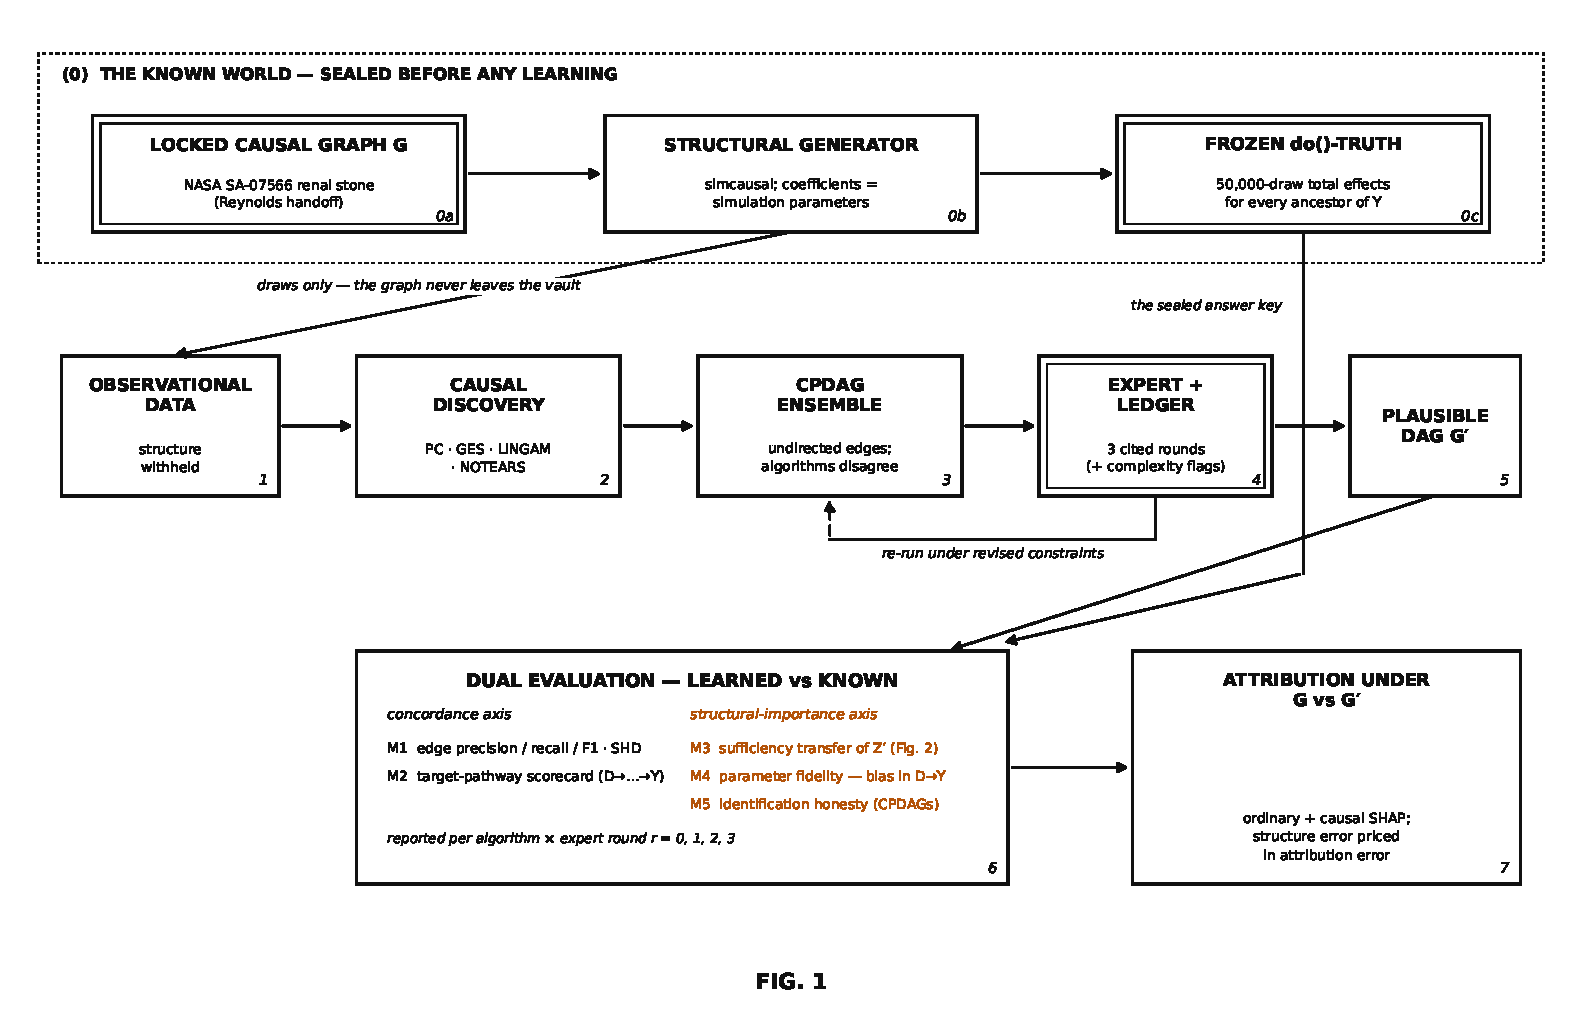
\includegraphics[width=\textwidth]{fig1_space_shap_spine.pdf}
\caption{The spine. Phase 0 is sealed before any learning; discovery,
ledger, and plausible graph follow; the learned graph is scored on a
concordance axis (M1, M2) and a structural-importance axis (M3 to M5)
before attribution is computed under both graphs.}
\label{fig:spine}
\end{figure}

\begin{figure}[htbp]
\centering
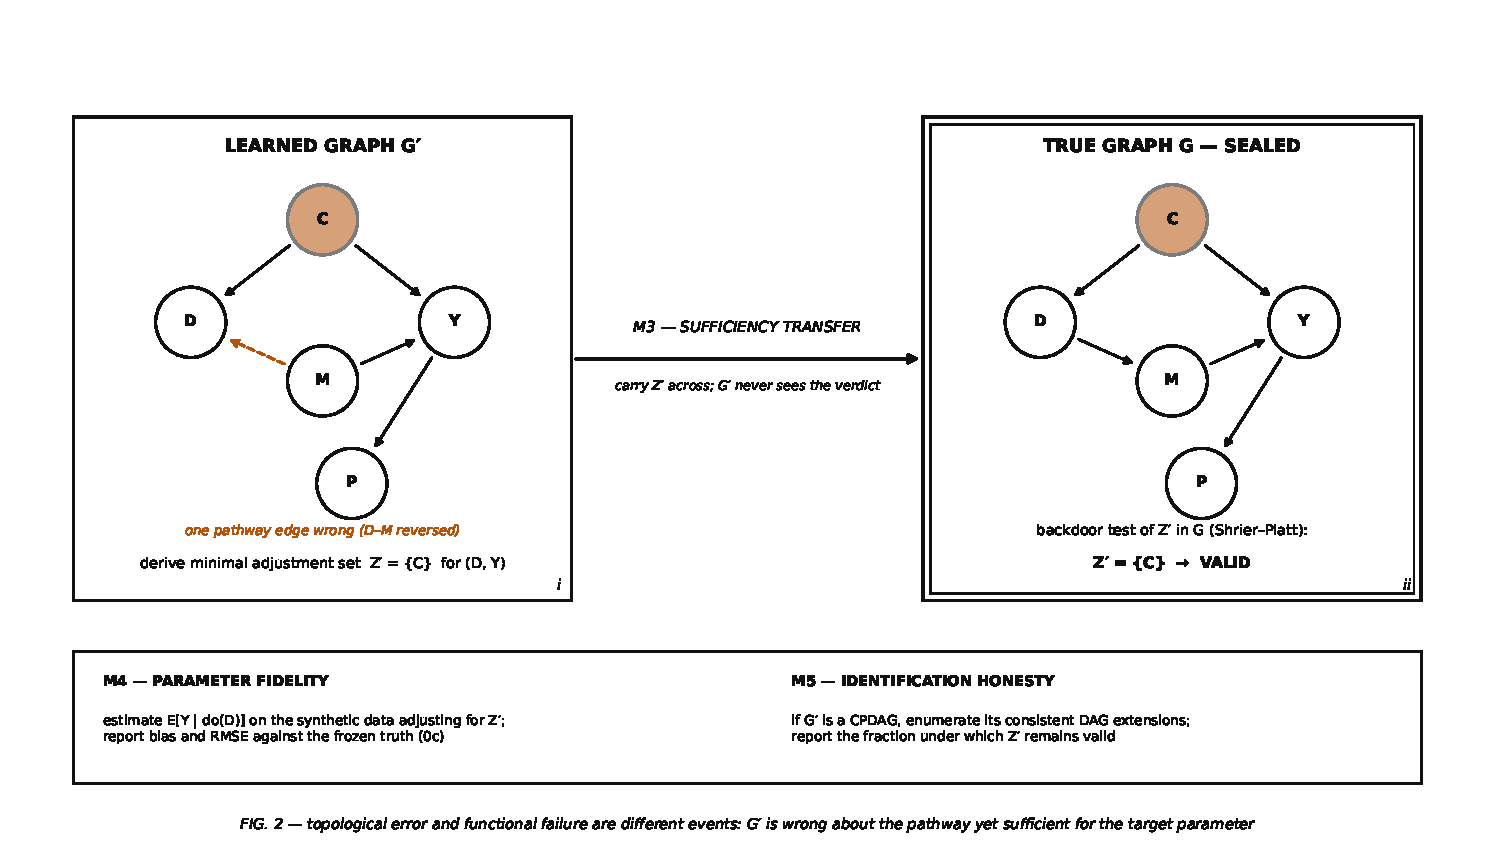
\includegraphics[width=\textwidth]{fig2_sufficiency_transfer.pdf}
\caption{Topological error and functional failure are different events. The
learned graph reverses one pathway edge yet its minimal adjustment set is
valid in the sealed graph.}
\label{fig:m3}
\end{figure}

\todo{Table: methods (PC, GES, DirectLiNGAM, NOTEARS; plus MGM PC-Stable) by
expert round, reporting M1 F1 and SHD, M2 pathway recovery, M3 validity and
Jaccard, M4 bias, M5 fraction. Pilot on the toy graph exists
(\texttt{analysis/run\_m1\_m5\_battery.py}); renal run pending.}

\subsection{The detector and the filter}
\draftnote{Steps 5 and 7; gated on Lucidity Sciences' sign-off, so this
subsection states the role and the interface and no results}

The playbook's third rung is a detector: a per-node signal drawn from the
fitted model's internal geometry rather than from its predictions, meant to
point at nodes whose predictive credit has been absorbed by something nearer
the outcome. The candidate is Lucidity Sciences' LumaWarp, a learned-kernel
classifier whose diagnostics expose a per-feature design vector. Its public
interface in this study fixes three channels per feature (depth, importance,
complexity), z-scored within each attribution group and flagged above one
standard deviation; which internal quantity feeds which channel, and the
observed behavior of those quantities, await the vendor's confirmation and
are not reported here. The fourth rung is a filter proposed by one of us
(L.P.): dichromatic sensitivity gating, two channels at different
sensitivities gated on their pattern of agreement, so that a single
threshold need not choose between missed deep nodes and admitted noise. Its
closest published relatives are two-stage screening \citep{FanLv2008} and
threshold selection against a null-control channel \citep{BarberCandes2015}.
Three prespecified experiments test both rungs: a two-layer tree (E1), a
three-layer tree (E2), and the same tree under shrinking $n$ and measurement
noise on the deep layers (E3).

% =====================================================================
\section{Discussion}
\draftnote{discussion}

The playbook is six rungs. Predict; explain; cast wider; filter; prune and
propagate; price. The prediction playbook stops at the second rung and, for
prediction, is right to. This study establishes the fifth rung's central
fact on two scales of one graph: supplying a causal ordering to the
attribution method changes nothing that survives a paired bootstrap, and
propagating interventions through the structural system does. It establishes
the second rung's failure at the scale that matters, a two-hop mediation
chain inverted by four of five predictive pairings. It documents, on the
discovery route, that a binary outcome can be pruned out of the learned graph
entirely at a realistic sample size and that the method built on that graph
then has no opinion at all. And it shows why the third and fourth rungs are
needed: the nodes the wider net is cast for are the ones sampling variance
erases first.

The working assumption running through the playbook is that direct
relationships tend to be linear. If the graph is drawn at the right
granularity, each direct edge is close enough to linear that the product
rule applies, the total effect of a deep node is computable from the edges
above it, and two candidate structures that imply different total effects
can be told apart from data already in hand. This is a modeling choice made
for identifiability \citep{Shimizu2006,Hoyer2009,Peters2017}, not a claim
about nature. We enforce it in the generating model, relax it in the
estimators wherever feasible, and price it in the robustness sweep with a
nonlinear generator.

The pruned, propagated ranking is an input to a decision, not the decision.
A target becomes an action only once feasibility and cost enter, and the
obvious objective, benefit per unit cost, is degenerate under linear costs.
The budget-constrained selection that replaces it, with benefit measured by
simulating $\dox(a)$ against the same exogenous draws, is implemented and
out of this article's scope \citep{Karimi2021,Karimi2020,Mothilal2020}.

\paragraph{Limitations.}
\begin{enumerate}
\item All datasets are synthetic. Topologies are source-aligned; coefficients
  are simulation parameters, not NASA estimates.
\item DAG-constrained ordering and structural intervention propagation answer
  different questions and should not share one label without stating the
  value function.
\item The structural result is a $32\times32\times32$ prototype without
  repeated-seed uncertainty over the full pipeline.
\item Rounds two and three of the expert loop are a scripted heuristic, not
  expert review; the design calls for the domain expert's revisions.
\item Discovery results are single-seed pilots. Skeleton recovery and directed
  recovery differ substantially.
\item The depth diagnostic is single-seed, derived from a proprietary runtime,
  and its internal semantics await the vendor's confirmation.
\item Intervention-target ranking is not a treatment recommendation. Safety,
  timing, reversibility, and domain constraints sit outside the engine.
\item Both estimation poles trust the same unverifiable input, the DAG. A
  wrong adjustment set makes a targeted estimate confidently wrong.
\item Attribution is not achievable effect; Shapley's efficiency axiom fixes
  the total to be divided.
\item The linearity assumption is stated and priced, not tested against
  mechanism.
\end{enumerate}

\paragraph{Future work.} Treatment-confounder feedback, a variable that is
both a baseline confounder and an exposure-driven mediator, motivates a
longitudinal sequel with g-methods \citep{Robins2000}; the working graph no
longer contains a concrete example. Cost-aware counterfactual recourse
(Step~13) is defined by its owners separately.

% =====================================================================
\section{Methods}
\draftnote{The Methods follow the 13-step flow of the original repository.
The prose below was assembled with an LLM from the project's plans and
records and must be rewritten by a human before submission. The pipeline
itself is the source of truth: \texttt{pipeline/}, \texttt{analysis/},
\texttt{apps/} in the repository.}

\subsection*{Overview and study design}
We evaluate whether causally informed feature-attribution methods recover
the true intervention-relevant importance of upstream risk factors more
faithfully than standard, causality-blind attribution, and whether iterative
human expert revision of the underlying causal structure improves that
recovery as data are degraded toward the constraints characteristic of
spaceflight epidemiology. The study is conducted on synthetic data generated
from a known causal structure, so that ground-truth feature importance is
defined by construction and every attribution method can be scored against
it. Steps 1 through 8 and 10 constitute the core analysis. Steps 9 and 11
are robustness and generalization extensions; Step 12 is future work; Step
13 is out of scope.

\subsection*{Step 1: Exposure and outcome specification}
The exposure is cumulative mission duration, operationalized as total days
in microgravity, chosen over a binary flown indicator or a mission-era
classification because it preserves the dose-response relationship central
to the mechanism: microgravity-induced bone resorption elevates circulating
and urinary calcium in proportion to exposure, which drives urinary
supersaturation and stone risk. The outcome is nephrolithiasis, the target
node of the published NASA DAG, as binary incidence with a logit link
throughout. Calcium-oxalate relative supersaturation (mineralized renal
material) is collapsed onto the outcome in the working subgraph
(Fig.~\ref{fig:dag}) and retained as an internal mediator in the full graph.

\subsection*{Step 2: Causal graph construction and expert-guided augmentation}
The base structure is the NASA HSRB SA-07566 renal-stone DAG, obtained in
DAGitty form through a domain-expert handoff and reconciled against the
publicly distributed source graph (after semantic node mapping: Cohen's
$\kappa$ 0.978, precision 1.000, recall 0.958, structural Hamming distance
3, with the unmatched edges retained for expert adjudication). The 14-node
working subgraph comprises the exposure, sex, a personal or family history
of nephrolithiasis (exogenous confounder), a hypercalciuria predisposition
(exogenous confounder feeding bone resorption and urinary calcium
excretion), in-flight vitamin D, dietary nutrient intake, urinary oxalate
excretion, bone formation and bone resorption (principal-component
composites of their biomarkers), parathyroid suppression, urinary calcium
excretion, hydration, a urine-chemistry composite, and the outcome. Nodes
that restrict cohort membership (astronaut selection) and the
countermeasure era are represented as sampling mechanisms stressed in
Step~10, not as graph nodes. Every edge carries an evidence status
(confirmed mechanism, magnitude estimate, direction only) following NASA's
level-of-evidence schema \citep{Ward2024}, and every augmentation is
reviewed by the domain expert before admission.

\subsection*{Step 3: Synthetic data generation}
Data are generated from the specified DAG with \texttt{simcausal}
\citep{Sofrygin2017}, entirely config-driven from the DAG specification and
a coefficient file. Coefficients are literature-informed placeholders
pending domain-expert calibration; where the literature supports only a
direction, the magnitude is recorded as an assumption to be varied. Binary
root nodes are mean-centered where they enter a downstream formula;
residual standard deviations are calibrated empirically so that
standardized nodes keep unit variance; the outcome intercept is calibrated
to a target prevalence. The default sample size is 1{,}000, the order of
magnitude of the astronaut corps, with larger samples where estimator
stability requires them. Because the simulations are linear-Gaussian with
additive noise, non-root nodes are standardized to remove the
variance-ordering leak that would otherwise favor discovery algorithms
\citep{Reisach2021}.

\subsection*{Step 4: Baseline attribution with standard SHAP}
Standard attributions are the reference. Expected attribution patterns are
first derived from the DAG in the spirit of testable implications
\citep{Reynolds2022}: because mediators are included alongside the exposure,
a causally faithful method should split the exposure's total effect into a
direct and a mediated component rather than double-count it. Five pairings
are run: interventional TreeExplainer on random forest and on XGBoost, a
closed-form LinearExplainer on logistic regression with the empirical
feature covariance, and KernelExplainer and PermutationExplainer on XGBoost
as a black box (a stacked ensemble was deferred). The link is logit
throughout; global importance is mean $|$SHAP$|$ on the held-out set.

\subsection*{Step 5: The detector}
Attribution outputs from Step~4 are passed to the depth detector. The
interface is public (an attribution table in the shared schema in; one row
per feature with three z-scored channels, flags, and provenance out); the
provider is external and gated. \todo{expand once sign-off clears}

\subsection*{Step 6: Causally informed attribution and human-in-the-loop iteration}
Four causally informed methods spanning full-graph-dependent to
structure-discovering are compared: causal Shapley values
\citep{Heskes2020}, implemented as an intervention-propagating coalition
value function; Shapley Flow \citep{Wang2021}, which attributes to edges;
asymmetric Shapley values \citep{Frye2020}, which need only a causal
ordering; and the discovery-based Causal SHAP of \citet{Ng2025}, which
infers a CPDAG with PC and quantifies edge strength with IDA before
attributing. XGBoost is the primary engine for all four so that engine
choice is not a second axis; the discovery-based method is additionally
run on random forest, its paper-native engine. Each method admits a
different kind of expert input: edge presence, direction, and functional
form for the graph-dependent methods; edge-level critique for Shapley Flow;
the ordering for asymmetric values; and orientation of undirected edges,
edge-weight correction, and the significance threshold for the
discovery-based method. Each method is run over three rounds, scored against
the frozen truth each round, with round-over-round stability recorded.

\subsection*{Step 7: The detector over Step 6}
Step~5's pass is repeated over the Step~6 outputs, under the same contract
and the same gate.

\subsection*{Step 8: Structural recovery comparison}
The discovery-based method's inferred graph is reused and structural
recovery is evaluated in its own right, one representative per family:
constraint-based (PC, reused; PC-stable \citep{ColomboMaathuis2014} and its
mixed-graphical-model form \citep{Sedgewick2019} because the outcome is
binary), score-based (GES \citep{Chickering2002}), continuous optimization
(NOTEARS \citep{Zheng2018}), and functional non-Gaussian (LiNGAM
\citep{Shimizu2006}). Each is scored on concordance (precision, recall, F1,
structural Hamming distance) and on structural importance: target-pathway
recovery, sufficiency transfer of the learned adjustment set into the sealed
graph, parameter fidelity of the exposure effect adjusted for that set, and
identification honesty over the CPDAG's consistent extensions. Recovery is
also reported as a function of node depth.

\subsection*{Step 9: Robustness to the data-generating process}
The narrowed pipeline of Steps 4 through 8 is re-run on data from
additional generators, including a nonlinear-edge generator that prices the
linearity assumption, and, should domain-restricted real data become
available, a real-data-seeded semi-synthetic validation in the spirit of
Credence \citep{Parikh2022}.

\subsection*{Step 10: Robustness to spaceflight-epidemiological constraints}
The narrowed pipeline is re-run under sampling regimes that emulate
spaceflight cohorts, applied as selection and degradation mechanisms rather
than as changes to the causal structure: reduced sample size, widened
mission-era ranges, selection on cardiovascular fitness and on a narrow age
window, and measurement noise on mediators. Attribution fidelity is tracked
as a function of the severity of each constraint.

\subsection*{Step 11: Generalization to out-of-distribution populations}
Reported in its own section: how attribution and prediction behave when the
target population differs structurally from the training population, for
example commercial-spaceflight participants or exploration-duration
missions.

\subsection*{Step 12: Longitudinal extension (future work)}
Treatment-confounder feedback motivates extending the static comparison to
a longitudinal setting with g-methods \citep{Robins2000}. Not undertaken.

\subsection*{Step 13: Counterfactual recourse extension (out of scope)}
A cost-aware counterfactual component, in which a complexity or cost score
defines the price of intervening on each feature, is a task distinct from
attribution and is left to its owners.

\subsection*{Evaluation metrics}
Attribution methods are scored against the frozen total effects with
Kendall's $\tau$, Spearman's $\rho$, top-$k$ recovery, and NDCG@$k$,
supplemented by the proximity-bias index (attribution-weighted mean directed
distance to the outcome under truth minus under the method), the proximal
over-attribution area (mean excess of the method's distance-concentration
curve over the truth's), and proximal mass within two hops. Structural
recovery is scored as in Step~8. Locked comparisons carry a paired bootstrap
over evaluation records.

\subsection*{Reproducibility and provenance}
All datasets are synthetic and contain no astronaut, patient, or participant
records. Graph topology is source-aligned to the published NASA DAG; all
coefficients are simulation design parameters. Data generation, attribution,
structural recovery, and evaluation are a scripted, version-controlled
pipeline with frozen output artifacts; the ground-truth total effects are
computed before and independently of the attribution comparison. Code,
frozen results, and this manuscript are at
\url{https://github.com/ahhatype/causal-shap-spaceflight-renal-stones};
the companion site is at
\url{https://andystats.github.io/causal-shap-target-dags/}.

\bibliographystyle{unsrtnat}
\bibliography{references}

\end{document}
